\documentclass{article}
\usepackage{hyperref}
\usepackage{graphicx}
\usepackage{float}
\usepackage{graphicx}
\usepackage[utf8]{inputenc}
\usepackage[T1]{fontenc}

\title{Analiza wypadków samochodowych w Polsce}
\author{Jakub Śliwka}
\date{15 May 2022}

\begin{document}

\maketitle

\section{Wstęp}
Polska jest jednym z czołowych krajów w Europie pod względem liczby śmiertelnych wypadków samochodowych w przeliczeniu na milion mieszkańców.
Pod tym względem tylko Rumunia, Bułgaria, Litwa i Chorwacja mają gorsze statystyki.
Wypadki drogowe są jedną z głównych przyczyn zgonów w Polsce. W kolejnych rozdziałach przybliżę temat wypadków samochodowych, przeanalizuję czynniki zewnętrzne takie 

\section{Analiza danych}
Dane zostały pobrane dzięki uprzejmości serwisów: \url{https://policja.pl/} oraz \url{https://danepubliczne.imgw.pl}.

Wykresy wypadków drogowych oraz danych pogodowych wyglądają dosyć podobnie. Oba wykresy przypominają sinusoidę.
Przede wszystkim można zauważyć, że wypadki drogowe zdarzają się najczęściej w okresie letnim, a najmniej w okresie zimowym.
Ilość osób rannych w wypadkach drogowych również przypomina sinusoidę. Wiąże się to z ilością wypadków drogowych.

\begin{figure}[h]
    \flushleft
    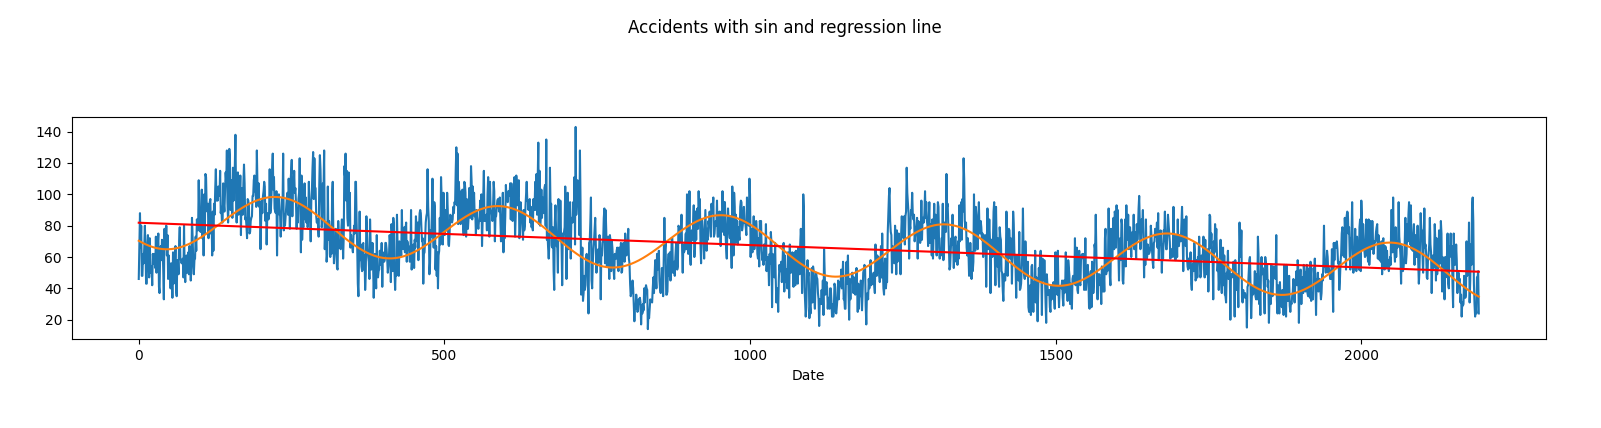
\includegraphics[width=1\textwidth]{visualization/accidents_sin.png}
    \caption{Wykres liczby wypadków drogowych z linią regresji oraz funkcją sinusoidalną}
    \label{fig:accidents_sin}
\end{figure}

\begin{figure}[h]
    \flushleft
    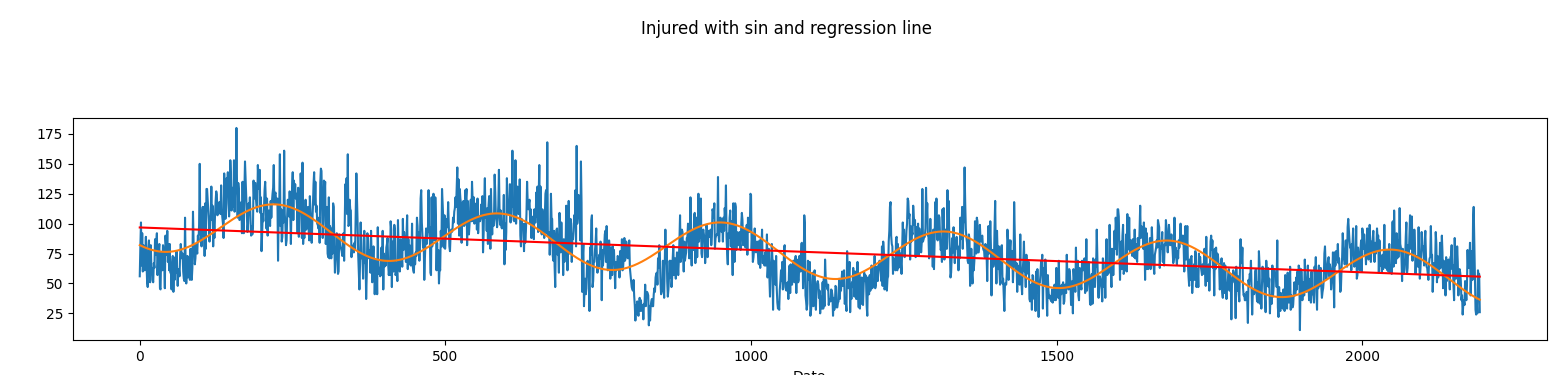
\includegraphics[width=1\textwidth]{visualization/injured_sin.png}
    \caption{Wykres poszkodowanych w wypadkach drogowych z linią regresji oraz funkcją sinusoidalną}
    \label{fig:injured_sin}
\end{figure}

\begin{figure}[h]
    \flushleft
    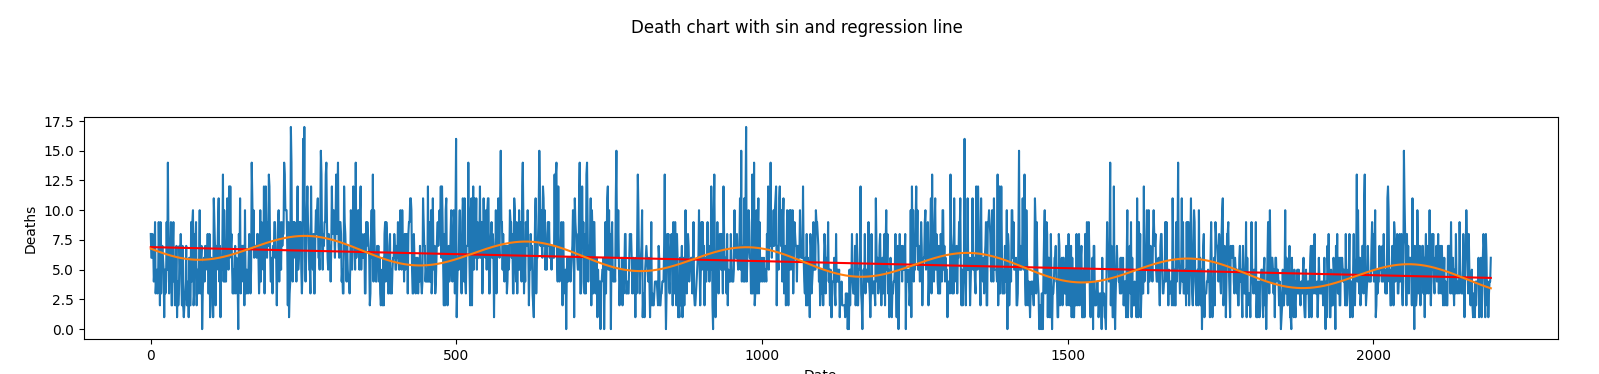
\includegraphics[width=1\textwidth]{visualization/death_sin.png}
    \caption{Wykres śmierci w wypadkach drogowych z linią regresji oraz funkcją sinusoidalną}
    \label{fig:death_sin}
\end{figure}

Na wszystkich trzech wykresach Data jest tak naprawdę ilością dni od 1 stycznia 2018 roku. 

Na wykresie \ref{fig:accidents_sin} możemy zauważyć tendencję spadkową w przeciągu ostatnich 5 lat. Wykres przypomina malejącą sinusoidę, którą w przybliżeniu można zaprezentować wzorem:

\begin{equation} \label{eq:sin_equation}
    y = -0.0143x + 81.884 + 20\sin(0.02x - 120) 
\end{equation}

Oczywiście funkcje przedstawione na wykresie są dużo dokładniejsze, a wzór \ref{eq:sin_equation} jest tylko przybliżeniem.

Podobinie sprawa ma się z wykresami \ref{fig:injured_sin} oraz \ref{fig:death_sin}. Oba wykresy przypominają sinusoidę, a wzory są podobne do wzoru \ref{eq:sin_equation}.
%cos wspomnieć o średniej lub stosunku śmierci/wypadków/rannych

\begin{equation} \label{eq:sin_equation_general}
    y = ax + b + c\sin(dx -e) 
\end{equation}
W tym miejscu można by było się zatrzymać i zakończyć analizę wypadków. Wzór ogólny \ref*{eq:sin_equation_general} wydaje się dokładnie odzwierciedlać rzeczywistość.
Na jego podstawie można by wysnuć tezę, że liczba wypadków z roku na rok maleje.
Co jeżeli obliczyć granicę ze wzoru \ref*{eq:sin_equation} przy x dążącym do nieskończoności?

\begin{equation} \label{eq:limit_sin}
    \lim_{x\to\infty}(-0.0143x + 81.884 + 20\sin(0.02x - 120))=-\infty
\end{equation}
Czy oznacza to, że wypadki drogowe w Polsce kiedyś znikną? Wypadków niestety nie da sie uniknąć, jednak nie zmienia to rzeczywistego faktu, że w Polsce 
liczba wypadków z roku na rok maleje. 


Jednak wypadki drogowe to nie tylko liczby, ale również ludzie i czynniki zewnętrzne. Warto zastanowić się nad tym, co jeszcze wpływa na ilość wypadków drogowych.

\section{Wpływ pogody na wypadki drogowe}

\subsection{Średnia temperatura powietrza}

Na poprzednich wykresach można było zauważyć korelację pomiędzy porami roku, a wypadkami samochodowymi.
Warto zobaczyć na wykres średniej dobowej temperatury w Polsce

\begin{figure}[h]
    \flushleft
    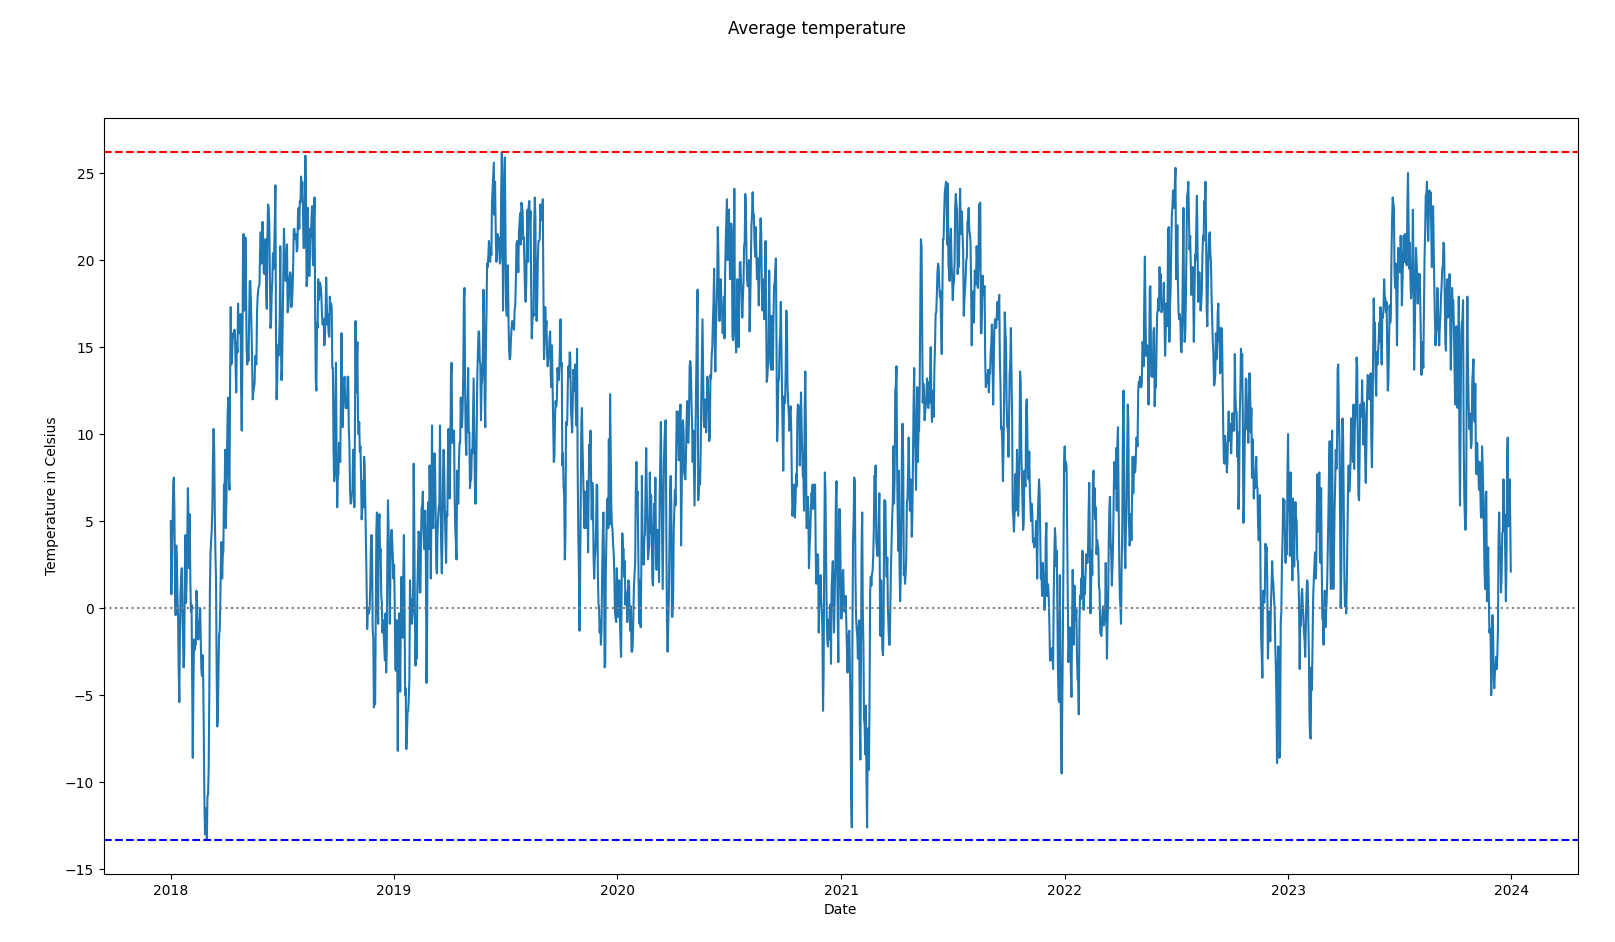
\includegraphics[width=1\textwidth]{visualization/avg_temp.png}
    \caption{Wykres średniej dobowej temperatury w Polsce w latach 2018-2023}
    \label{fig:temp_chart}
\end{figure}

% wykres średniej dobowej temperatury
Z łatwością można zauważyć, że wykres ten jest mocno zbliżony do wykresu przedstawiającego wypadki w Polsce.
Dlaczego akurat lato jest najbardziej niebezpieczną porą roku? Odpowiedź jest banalnie prosta. 
Ładna pogoda, usypia czujność kierowców. W trudniejszych warunkach jakie panuja zimą, od kierowców wymagane jest ciągłe skupienie.

% subsub sub section opady
\subsection{Opady atmosferyczne}

Czy opady atmosferyczne powodują większą ilośc wypadków samochodowych na drogach?

\begin{figure}[h]
    \flushleft
    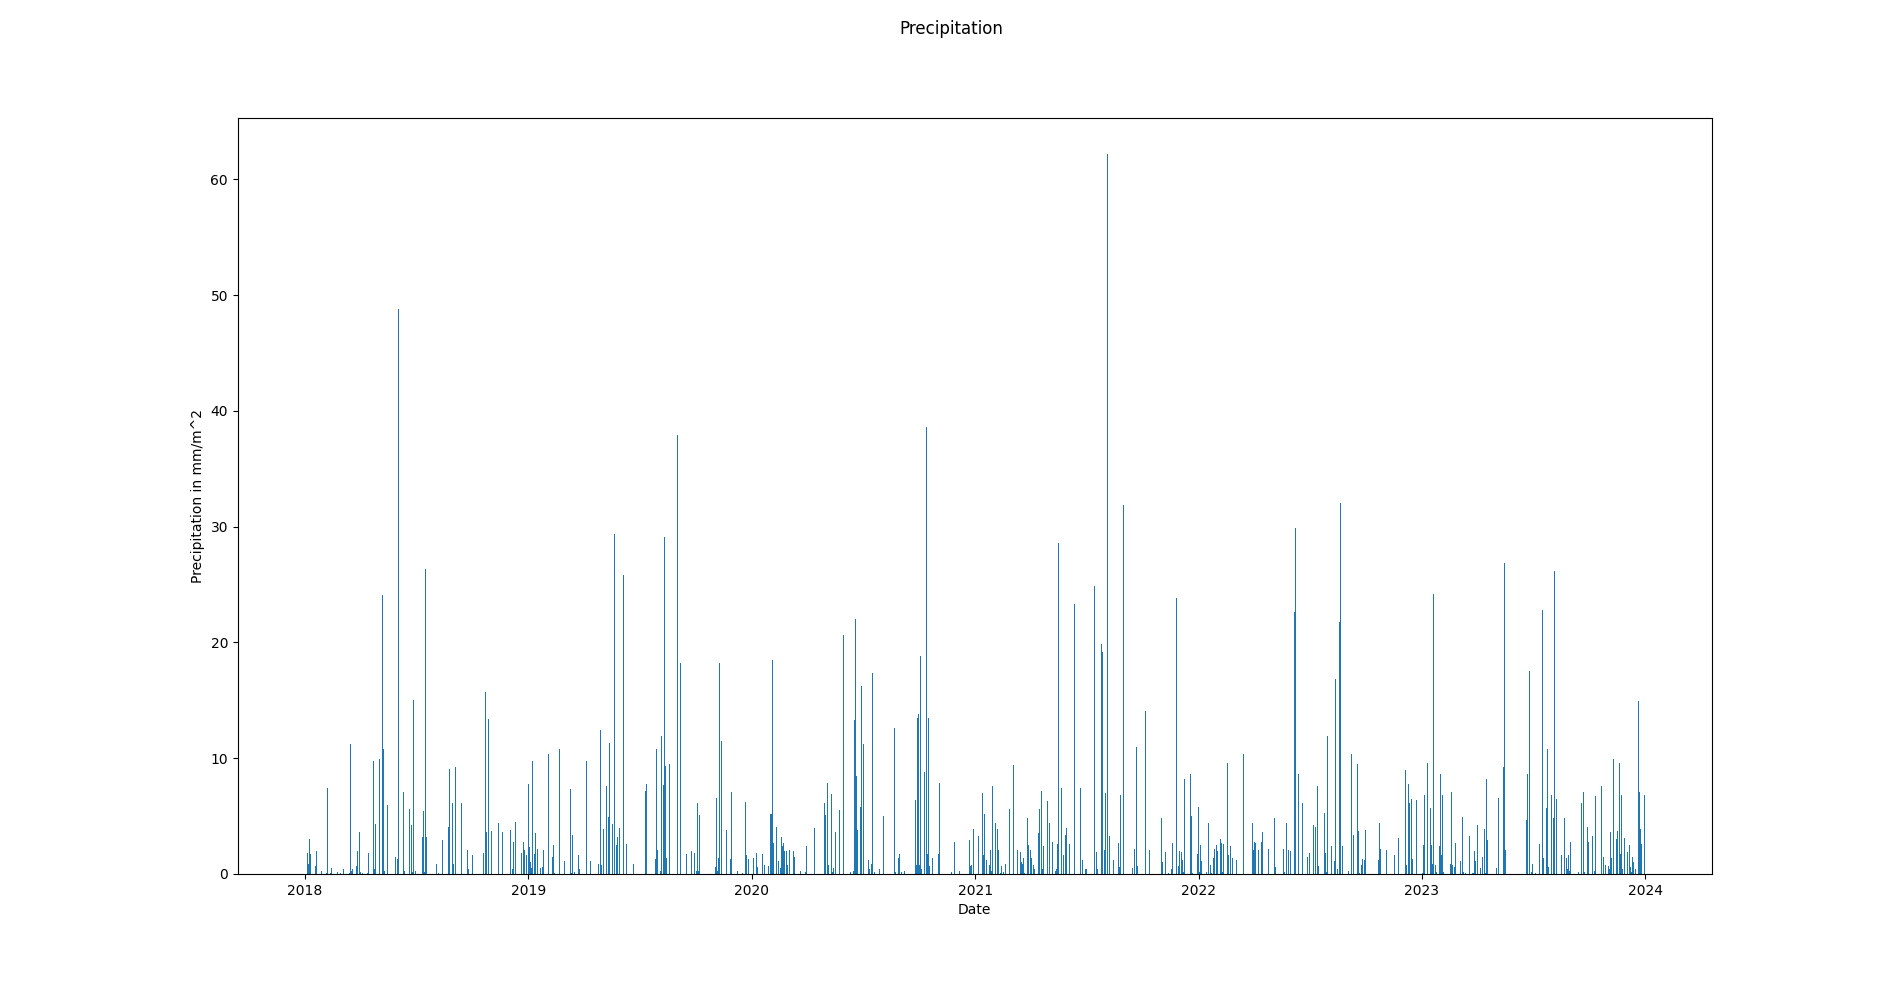
\includegraphics[width=1\textwidth]{visualization/precips.png}
    \caption{Wykres opadów w Polsce w latach 2018-2023 }
    \label{fig:precip_chart}
\end{figure}
% wykres opadów atmosferycznych
Na pierwszy rzut oka trudno doszukiwac się jakiś korelacji pomiędzy opadami a wypadkami
% coś tam o stosunku wypadków w deszczu a bez deszczu
\subsubsection{Opady atmosferyczne - deszcz}
% wykres opadów desczu
BLA BLA BLA TODO 
\subsubsection{Opady atmosferyczne - śnieg}
% wykres opadów śniegu
W przypadku opadów śniegu trudno doszukiwac się jakiejkolwiek korelacji. Ilość opadów jest mała w porównaniu z opadami desczu w Polsce. 
Ponadto w podczas zimy jak wczesniej było wspomniane, jest dużo mniej wypadków niż w czasie lata, co utrudnia anaizę tych danych. 
\subsubsection{Opady deszczu a opady śniegu}
% stosunek wypadków w desczu i śniegu TODO
Bla bla bla TODO 
% SECTION LUB SUBSECTION Co jeszcze może mieć wpływ na wypadki w Polsce

Weekendy oraz święta. 
% TODO stosunki świąt i weekendów do siebie czy coś 

%jjakiś nagłówek czy coś
Po tak wielu czynnikach jakimi są zmienna pogoda, święta oraz weekendy, czy da się na ich podstawie przewidzieć ilość wypadków, rannych oraz śmierci w Polsce?
To zagadnienie zostanie omówione w kolejnym rozdziale.

\section{Predykcja wypadków w Polsce}

Ze względu na rodzaj danych zdecydowałem się na wybór \textit{Regressor}'ów. Moim celem jest przewidzenie dokładnej ilości wypadków przy odpowiednich warunkach.



\section{Zakończenie}

Jak widac 

\end{document}
